\documentclass[a4paper]{article}

  \usepackage{fullpage} % Package to use full page
  \usepackage{parskip} % Package to tweak paragraph skipping
  \usepackage{tikz} % Package for drawing
  \usepackage{amsmath}
  \usepackage{siunitx}
  \usepackage{amsfonts}
  \usepackage{amssymb}
  \usepackage{hyperref}
  \usepackage[utf8]{inputenc}
  \usepackage[english]{babel}
  \usepackage{multicol}
  \usepackage{graphicx}
  \graphicspath{ {./images/} }
  
  \newcommand\tab[1][0.5cm]{\hspace*{#1}}
  
  \title{Laboratory 2: Resistor Combinations, KCL, KVL, Voltage and Current Dividers}
  \author{Adrian Darian, Elaine Huang, Federico Del Castillo Carnero}
  \date{9/16/2020}
  
  \begin{document}
  
\maketitle
  
\section*{Objectives}
\begin{itemize}
	\item Verify KCL and KVL
	\item Measure resistor combinations
	\item Measure branch currents and node voltages
\end{itemize}

\section*{Equipment and Components}
\begin{itemize}
	\item A computer
	\item Matlab software
\end{itemize}

\section*{Preliminary}
\begin{itemize}
	\item[1.] Refer to Chapters 2 and 3 of the textbook if necessary.
	\item[2.] Complete the theoretical calculations related to this lab. 
\end{itemize}

\section*{Procedure}
\begin{itemize}
	\item[1] Open Matlab
	\item[2] Create Simulink model of the circuit shown below by following the procedure in Lab 1
	\item[3] Fill up your simulation results in the following table. \\
	      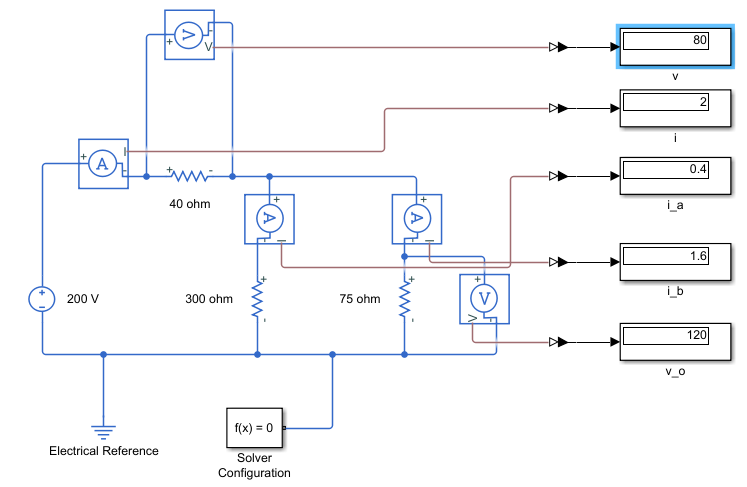
\includegraphics[scale=0.5]{circuit-1+200.png} \\
	      \begin{tabular}{|c|c|c|}
	      	\hline
	      	Source $= 200 V$ & Simulation Results & Theoretical Results \\
	      	\hline
	      	$i$              & $2A$               & $2A$                \\
	      	\hline
	      	$i_{a}$          & $0.4A$             & $0.4A$              \\
	      	\hline
	      	$i_{b}$          & $1.6A$             & $1.6A$              \\
	      	\hline
	      	$v$              & $80V$              & $80V$               \\
	      	\hline
	      	$v_{o}$          & $120V$             & $120V$              \\
	      	\hline
	      \end{tabular} 
	      \begin{tabular}{rcl}
	      	$i_{a}$ & $=$ & $\frac{v_{o}}{R_{a}}$                                                    \\
	      	        & $=$ & $\frac{120}{300}$                                                        \\
	      	        & $=$ & $0.4A$                                                                   \\
	      	$i_{b}$ & $=$ & $\frac{v_{o}}{R_{b}}$                                                    \\
	      	        & $=$ & $\frac{120}{75}$                                                         \\
	      	        & $=$ & $1.6A$                                                                   \\
	      	$i$     & $=$ & $i_{a} + i_{b}$                                                          \\
	      	        & $=$ & $2A$                                                                     \\
	      	$v_{o}$ & $=$ & $\frac{v_{o} - v_{g}}{R{g}} + \frac{v_{o}}{R_{a}} + \frac{v_{o}}{R_{b}}$ \\
	      	        & $=$ & $120V$                                                                   \\
	      	$v$     & $=$ & $v_{s} - v_{o}$                                                          \\
	      	        & $=$ & $80V$                                                                    \\
	      \end{tabular}
	      \begin{itemize}
	      	\item[a.] What is the sum of $i_{a}$ and $i_{b}$? Sum $= 2$. What is $i$? Explain. \\
	      	      \textbf{Answer:} $i$ is the initial current flowing out of the voltage source. Also Current does not change when passing through resistors it only splits at forks in the ciruit.
	      	\item[b.] What is the sum of $v$ and $v_{o}$? Sum $= 200$. Explain.
	      	\item[c.] Are your simulation results consistent with your theoretical results of Problem 2.18 in Assignment 2?
	      	\item[d.] Set the voltage source to be $100 V$ and repeat the above steps. Fill up the table below. Comparing the results in Table 2 with those in Table 1, what do you find? \\
	      	      \textbf{Answer:} We found that when comparing the results between a $200V$ and a $100V$ source the $100V$ is exactly half the readings of the $200V$   
	      \end{itemize}
	      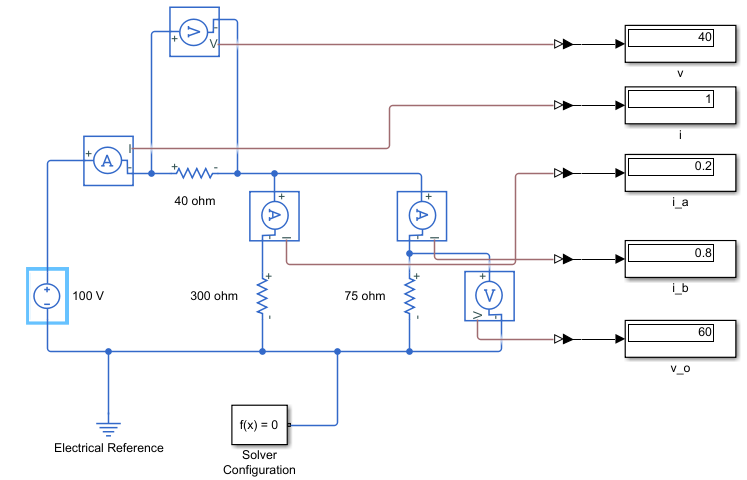
\includegraphics[scale=0.5]{circuit-1+100.png}\\
	      \begin{tabular}{|c|c|c|}
	      	\hline
	      	Source $= 100 V$ & Simulation Results & Theoretical Results \\
	      	\hline
	      	$i$              & $1A$               & $1A$                \\
	      	\hline
	      	$i_{a}$          & $0.2A$             & $0.2A$              \\
	      	\hline
	      	$i_{b}$          & $0.8A$             & $0.8A$              \\
	      	\hline
	      	$v$              & $40V$              & $40V$               \\
	      	\hline
	      	$v_{o}$          & $60V$              & $60V$               \\
	      	\hline
	      \end{tabular} 
	      \begin{tabular}{rcl}
	      	$i_{a}$ & $=$ & $\frac{v_{o}}{R_{a}}$                                                    \\
	      	        & $=$ & $\frac{120}{300}$                                                        \\
	      	        & $=$ & $0.2A$                                                                   \\
	      	$i_{b}$ & $=$ & $\frac{v_{o}}{R_{b}}$                                                    \\
	      	        & $=$ & $\frac{120}{75}$                                                         \\
	      	        & $=$ & $0.8A$                                                                   \\
	      	$i$     & $=$ & $i_{a} + i_{b}$                                                          \\
	      	        & $=$ & $1A$                                                                     \\
	      	$v_{o}$ & $=$ & $\frac{v_{o} - v_{g}}{R{g}} + \frac{v_{o}}{R_{a}} + \frac{v_{o}}{R_{b}}$ \\
	      	        & $=$ & $60$                                                                     \\
	      	$v$     & $=$ & $v_{s} - v_{o}$                                                          \\
	      	        & $=$ & $40$                                                                     \\
	      \end{tabular}
	      \begin{itemize}
	      	\item[e.] Set the voltage source to be $-200V$ repeat the above steps 1, 2, and 3. Fill up the table below. Comparing the results in Table 3 with those in Table 1, what do you find? \\
	      	      \textbf{Answer:} We found that when comparing the results between a $200V$ and a $-200V$ source the $-200V$ contains the same results except negative of the $200V$
	      \end{itemize}
	      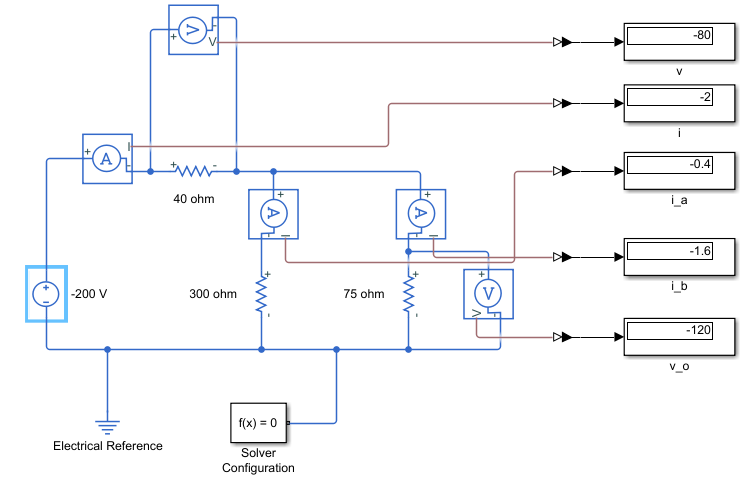
\includegraphics[scale=0.5]{circuit-1-200.png} \\
	      \begin{tabular}{|c|c|c|}
	      	\hline
	      	Source $= -200 V$ & Simulation Results & Theoretical Results \\
	      	\hline
	      	$i$               & $-2A$              & $-2A$               \\
	      	\hline
	      	$i_{a}$           & $-0.4A$            & $-0.4A$             \\
	      	\hline
	      	$i_{b}$           & $-1.6A$            & $-1.6A$             \\
	      	\hline
	      	$v$               & $-120V$            & $-120V$             \\
	      	\hline
	      	$v_{o}$           & $-120V$            & $-120V$             \\
	      	\hline
	      \end{tabular} 
	      \begin{tabular}{rcl}
	      	$i_{a}$ & $=$ & $\frac{v_{o}}{R_{a}}$                                                    \\
	      	        & $=$ & $\frac{120}{300}$                                                        \\
	      	        & $=$ & $-0.4A$                                                                  \\
	      	$i_{b}$ & $=$ & $\frac{v_{o}}{R_{b}}$                                                    \\
	      	        & $=$ & $\frac{120}{75}$                                                         \\
	      	        & $=$ & $-1.6A$                                                                  \\
	      	$i$     & $=$ & $i_{a} + i_{b}$                                                          \\
	      	        & $=$ & $-2A$                                                                    \\
	      	$v_{o}$ & $=$ & $\frac{v_{o} - v_{g}}{R{g}} + \frac{v_{o}}{R_{a}} + \frac{v_{o}}{R_{b}}$ \\
	      	        & $=$ & $-120V$                                                                  \\
	      	$v$     & $=$ & $v_{g} - v_{o}$                                                          \\
	      	        & $=$ & $-80V$                                                                   \\
	      \end{tabular}
	\item[4] Create the Simulink of the following circuit and find $i_{g}$ and $i_{o}$. Fill up the table shown below. Are the simulation solutions with your theoretical solutions of Problem 3.28 in Assignment 3? 
	      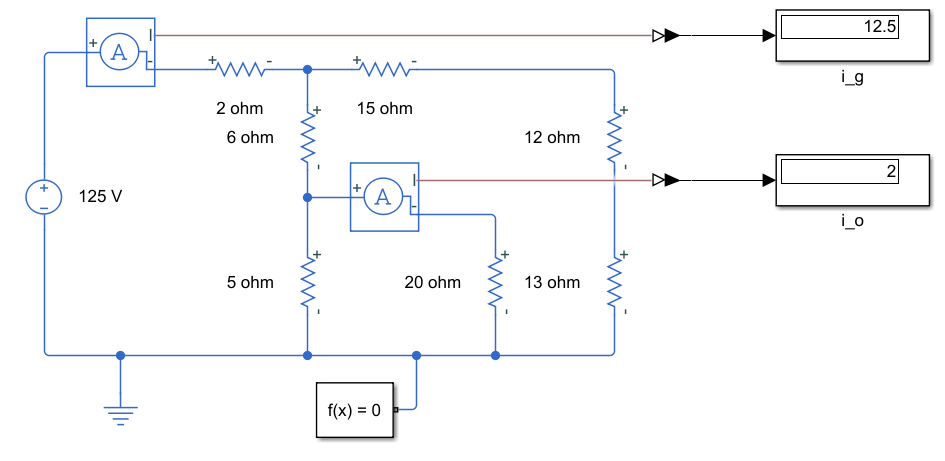
\includegraphics[scale=0.5]{circuit-2.png} \\
	      \begin{tabular}{|c|c|c|}
	      	\hline
	      	        & Simulation Results & Theoretical Results \\
	      	\hline
	      	$i_{g}$ & $12.5A$            & $12.5A$             \\
	      	\hline
	      	$i_{o}$ & $2A$               & $2A$                \\
	      	\hline
	      \end{tabular} 
	      \begin{tabular}{rcl}
	      	$i_{i}$ & $=$ & $\frac{i_{g} * (12 + 13 + 15)}{10 + (12 + 13 + 15)}$ \\
	      	        & $=$ & $10A$                                                \\
	      	$i_{o}$ & $=$ & $\frac{i_{i} * 5}{20 + 5}$                           \\
	      	        & $=$ & $2A$                                                 \\
	      	$i_{g}$ & $=$ & $\frac{125}{2 + 8}$                                  \\
	      	        & $=$ & $12.5A$                                              \\
	      \end{tabular}
	\item[5] Create the Simulink model of the following circuit and find $v_{1}$ and $v_{2}$. Are the simulation solutions consistent with your theoretical solutions of Problem 3.30 in Assignment 3? Fill up the table shown below. \\
	      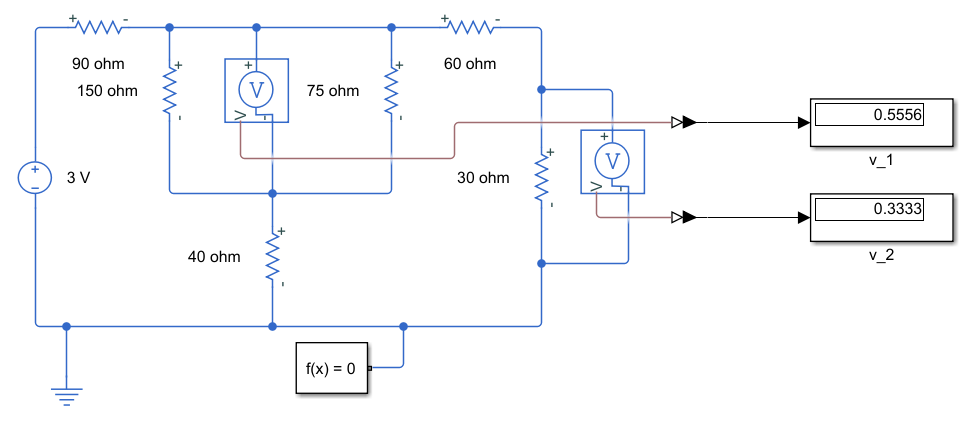
\includegraphics[scale=0.5]{circuit-3.png} \\      
	      \begin{tabular}{|c|c|c|}
	      	\hline
	      	        & Simulation Results & Theoretical Results \\
	      	\hline
	      	$v_{1}$ & $0.5556V$          & $0.5556V$           \\
	      	\hline
	      	$v_{2}$ & $0.3333V$          & $0.3333V$           \\
	      	\hline
	      \end{tabular} 
	      \begin{tabular}{rcl}
	      	$v_{1}$ & $=$ & $(150 ||75)||((150||75) + 40)$ \\
	      	        & $=$ & $0.5556V$                      \\
	      	$v_{2}$ & $=$ & $\frac{30}{30 + 60}$           \\
	      	        & $=$ & $0.3333V$                      \\
	      \end{tabular}
\end{itemize}

\section*{Questions and Conclusions}
\begin{itemize}
	\item Use tables and graphs to explain your results.
	\item Summarize your findings and explanations in response to the questions posed in this lab. \\
	\textbf{Answer:} The first few circuit diagrams we created in lab allowed us to observe the change in voltage and current across the whole system, through changing the voltage source potential. In the 2nd circuit we got to observe the change in current and found that the current drastically decreased as the voltage passed through the circuit. In the 3rd circuit we got to observe the change in voltage as we added more resistors in series and in parallel to the circuit diagram. 
\end{itemize}

% ehuang34@ucmerced.edu
% fdelcastillo@ucmerced.edu
  
\end{document}